% !Mode::"TeX:UTF-8"
\documentclass[a4paper, 10pt]{article}
\usepackage{amssymb}
\usepackage{geometry}
\usepackage{graphicx}
\usepackage{fancyhdr}
\usepackage{setspace}
\usepackage{pdfpages}
\usepackage{listings}
\usepackage{amsthm}
\usepackage{authblk}
\usepackage{amsmath}
\usepackage{url}
\usepackage{hyperref}

\graphicspath{{./figure/}}

\geometry{left=2.5cm,right=2.5cm,top=2.5cm,bottom=2.5cm}

%\author{Chi Zhang\\\\Department of Computer Science\\\\University of Southern California}
\title{\textbf{Deep Reinforcement Learning for Portfolio Management}\thanks{Instructor: Joseph J. Lim}}
\author[]{Chi Zhang}
\author[]{Limian Zhang}
\author[]{Corey Chen}
\affil[]{Department of Computer Science}


\begin{document}

  \maketitle                     %generate the title
  \begin{spacing}{1.2}
    \section{Problem Definition}
    \subsection{Notations}
    In this project, we would like to manage portfolio by distributing our investment into a number of stocks based on the market. We define our environment similar to this paper \cite{DBLP:journals/corr/JiangXL17}.
    Concretely, we define $N$ to be the number of stocks we would like to invest.
    Without losing generality, at initial timestamp, we assume our total investment volume is 1 dollar. We define \emph{close/open relative price vector} as:
    \begin{equation}
    y_t=[1, \frac{v_{1,t, close}}{v_{1,t, open}}, \frac{v_{2,t, close}}{v_{2,t, open}},\cdots,\frac{v_{N,t,close}}{v_{N,t, open}}]
    \end{equation}
    where $\frac{v_{i, t, close}}{v_{i, t, open}}$ is the \emph{relative price} of stock $i$ at timestamp $t$. 
    Note $y[0]$ represents the relative price of cash, which is always 1. We define \emph{portfolio weight vector} as:
    \begin{equation}
    w_t=[w_{0,t}, w_{1, t}, \cdots, w_{N, t}]
    \end{equation}
    where $w_{i,t}$ represents the fraction of investment on stock $i$ at timestamp $t$. Note that $w_{0,t}$ represents the fraction of cash that we maintain. Then the profit after timestamp $T$ is:
    \begin{equation}
    \label{profit}
    p_T=\prod_{t=1}^{T}y_t\cdot w_{t-1}
    \end{equation}
    where $w_0=[1, 0, \cdots, 0]$. If we consider a trading cost factor $\mu$, then the trading cost of each timestamp is:
    \begin{equation}
    {\mu}_t=\mu\sum{|\frac{y_t \odot w_{t-1}}{y_t \cdot w_{t-1}} - w_{t}|}
    \end{equation}
    where $\odot$ is element-wise product. Then equation~\ref{profit} becomes:
    \begin{equation}
    \label{profit_mu}
    p_T=\prod_{t=1}^{T}(1-\mu_t) y_t\cdot w_{t-1}
    \end{equation}
    
    \subsection{Key Assumptions and Goal}
    To model real world market trades, we make several assumptions to simplify the problems:
    \begin{itemize}
      \item We can get any information about the stocks before timestamp $t$ for stock $i$. e.g. The previous stock price, the news and tweets online.
      \item Our investment will not change how the market behaves.
      \item The way we calculate profit in equation~\ref{profit} can be interpreted as: At timestamp $t$, we buy stocks according to the \emph{portfolio weight vector} $w_{t-1}$ computed by history data at \textbf{open} price and sell all the stocks at \textbf{close} price. This may not be true in practice because you will not always be able to \textbf{buy/sell} the stock at \textbf{open/close} price.
    \end{itemize}
    The \textbf{goal} of portfolio management is to maximum $p_T$ by choosing portfolio weight vector $w$ at each timestamp $t$ based on history stock information.
    
    \subsection{MDP formulation}
    \subsubsection{State and Action}
    We define state $s_t$ as $(o_t, a_{i-1})$ pair, where $o_t$ is the obseration of timestamp $t$. Since we can't feed variable length data into CNN/LSTM models, we only consider the history price in a window length $W$. Thus,
    \begin{equation}
    o_t=[\vec{v_{1,t}},\vec{v_{2,t}},\cdots,\vec{v_{N,t}}]
    \end{equation}
    where
    \begin{align}
    v_{i,t} &=\begin{bmatrix}
    v_{i,t-W+1} \\
    v_{i,t-W+2} \\
    \vdots \\
    v_{i,t}
    \end{bmatrix}
    \end{align}
    The action $a_{i-1}$ is just \emph{portfolio weight vector} $w_{i-1}$. In this problem, we would like to train a policy network $\pi_{\theta}(a_t|s_t)=\pi_{\theta}(a_t|o_t,a_{t-1})$. We will directly use $s_t=(o_t, a_{i-1})$ in our following discussion.\\
    \subsubsection{State Transition}
    The underlining state evolution is determined by the market, which we don't have any control. What we can get is the observation state, which is the price. Since we will collect history price of various stocks, $o_t$ is given by the dataset instead of $o_{t-1}$.\\
    \subsubsection{Reward}
    Instead of having reward 0 at each timestamp and $p_T$ at the end, we take logarithm of equation~\ref{profit_mu}:
    \begin{equation}
    \log{p_T}=\log{\prod_{t=1}^{T}\mu_t y_t\cdot w_{t-1}}=\sum_{t=1}^{T}\log(\mu_t y_t\cdot w_{t-1})
    \end{equation}
    Thus, we have $\log(\mu_t y_t\cdot w_{t-1})$ reward each timestamp, which avoids the sparsity of reward problem.\\
    \subsubsection{Discount Factor}
    The discount factor $\gamma$ is 1 because future rewards are as important as current rewards.
    
    \subsection{Datasets}
    \textbf{Price Data:}
    We collected history price of 16 stocks from 2012-08-13 to 2017-08-11. The price on each day contains (open, high, low, close, volume). We use 2012-08-13 to 2015-08-12 as training data and 2015-08-13 to 2017-08-11 as testing data.\\
    \textbf{News Data:}
    
    \section{Methods}
    We consider both model-free and model-based approach. The main difference is that in model-based approach, we try to predict the open and close price of future timestamp before making actions. In model-free approach, we try to learn policy $\pi_{\theta}(a_t|s_t)$ directly from history data.
    \subsection{Deep Deterministic Policy Gradient}
    
    
    \subsection{Model-based Approach}
    \subsubsection{Price Prediction}
    
    \subsubsection{Planning}
    
    \subsubsection{End-to-End training}
    
    \section{Results and Discussions}
    
%    
%    \begin{figure}
%      \centering
%      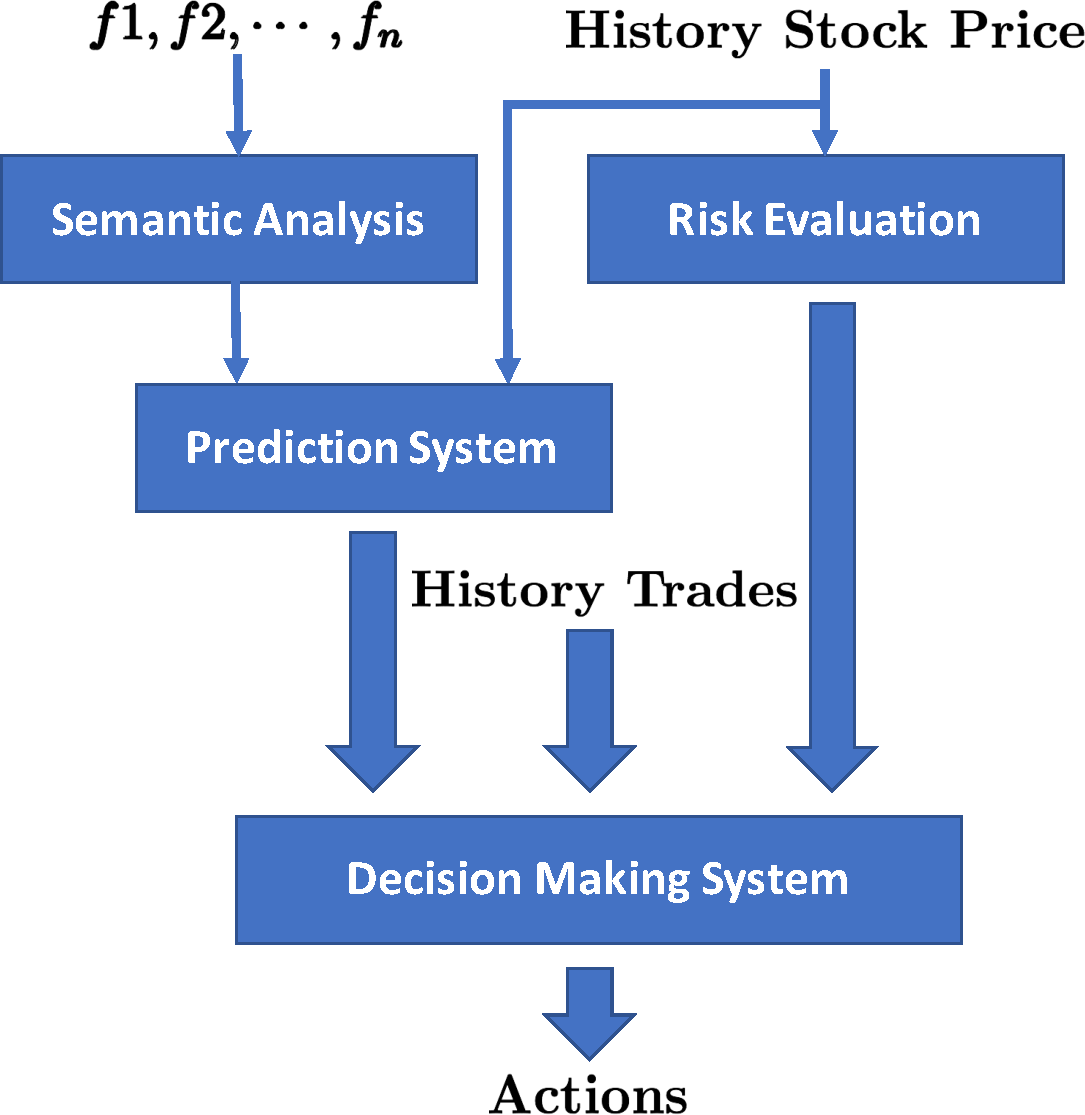
\includegraphics[width=0.4\textwidth]{diagram}
%      \caption{Digram of proposed approach}
%      \label{diagram_approach}
%    \end{figure}
    
    
  
  \end{spacing}  
  \bibliographystyle{abbrv}
  \bibliography{./bib/stock_prediction.bib}

\end{document}
